% Options for packages loaded elsewhere
\PassOptionsToPackage{unicode}{hyperref}
\PassOptionsToPackage{hyphens}{url}
\PassOptionsToPackage{dvipsnames,svgnames,x11names}{xcolor}
%
\documentclass[
  11pt,
]{book}
\usepackage{amsmath,amssymb}
\usepackage{lmodern}
\usepackage{iftex}
\ifPDFTeX
  \usepackage[T1]{fontenc}
  \usepackage[utf8]{inputenc}
  \usepackage{textcomp} % provide euro and other symbols
\else % if luatex or xetex
  \usepackage{unicode-math}
  \defaultfontfeatures{Scale=MatchLowercase}
  \defaultfontfeatures[\rmfamily]{Ligatures=TeX,Scale=1}
\fi
% Use upquote if available, for straight quotes in verbatim environments
\IfFileExists{upquote.sty}{\usepackage{upquote}}{}
\IfFileExists{microtype.sty}{% use microtype if available
  \usepackage[]{microtype}
  \UseMicrotypeSet[protrusion]{basicmath} % disable protrusion for tt fonts
}{}
\makeatletter
\@ifundefined{KOMAClassName}{% if non-KOMA class
  \IfFileExists{parskip.sty}{%
    \usepackage{parskip}
  }{% else
    \setlength{\parindent}{0pt}
    \setlength{\parskip}{6pt plus 2pt minus 1pt}}
}{% if KOMA class
  \KOMAoptions{parskip=half}}
\makeatother
\usepackage{xcolor}
\IfFileExists{xurl.sty}{\usepackage{xurl}}{} % add URL line breaks if available
\IfFileExists{bookmark.sty}{\usepackage{bookmark}}{\usepackage{hyperref}}
\hypersetup{
  pdftitle={Transforming Research Methods in Health Services Psychology: Applications for the Advocate \textasciitilde{} Practitioner \textasciitilde{} Scientist},
  pdfauthor={Lynette H. Bikos, PhD, ABPP},
  colorlinks=true,
  linkcolor={Maroon},
  filecolor={Maroon},
  citecolor={Blue},
  urlcolor={blue},
  pdfcreator={LaTeX via pandoc}}
\urlstyle{same} % disable monospaced font for URLs
\usepackage[margin=1in]{geometry}
\usepackage{longtable,booktabs,array}
\usepackage{calc} % for calculating minipage widths
% Correct order of tables after \paragraph or \subparagraph
\usepackage{etoolbox}
\makeatletter
\patchcmd\longtable{\par}{\if@noskipsec\mbox{}\fi\par}{}{}
\makeatother
% Allow footnotes in longtable head/foot
\IfFileExists{footnotehyper.sty}{\usepackage{footnotehyper}}{\usepackage{footnote}}
\makesavenoteenv{longtable}
\usepackage{graphicx}
\makeatletter
\def\maxwidth{\ifdim\Gin@nat@width>\linewidth\linewidth\else\Gin@nat@width\fi}
\def\maxheight{\ifdim\Gin@nat@height>\textheight\textheight\else\Gin@nat@height\fi}
\makeatother
% Scale images if necessary, so that they will not overflow the page
% margins by default, and it is still possible to overwrite the defaults
% using explicit options in \includegraphics[width, height, ...]{}
\setkeys{Gin}{width=\maxwidth,height=\maxheight,keepaspectratio}
% Set default figure placement to htbp
\makeatletter
\def\fps@figure{htbp}
\makeatother
\setlength{\emergencystretch}{3em} % prevent overfull lines
\providecommand{\tightlist}{%
  \setlength{\itemsep}{0pt}\setlength{\parskip}{0pt}}
\setcounter{secnumdepth}{5}
\usepackage{booktabs}
\ifLuaTeX
  \usepackage{selnolig}  % disable illegal ligatures
\fi
\usepackage[]{natbib}
\bibliographystyle{plainnat}

\title{Transforming Research Methods in Health Services Psychology: Applications for the Advocate \textasciitilde{} Practitioner \textasciitilde{} Scientist}
\author{Lynette H. Bikos, PhD, ABPP}
\date{27 Jun 2022}

\begin{document}
\maketitle

{
\hypersetup{linkcolor=}
\setcounter{tocdepth}{3}
\tableofcontents
}
\hypertarget{book-cover}{%
\chapter*{BOOK COVER}\label{book-cover}}
\addcontentsline{toc}{chapter}{BOOK COVER}

\begin{figure}
\centering
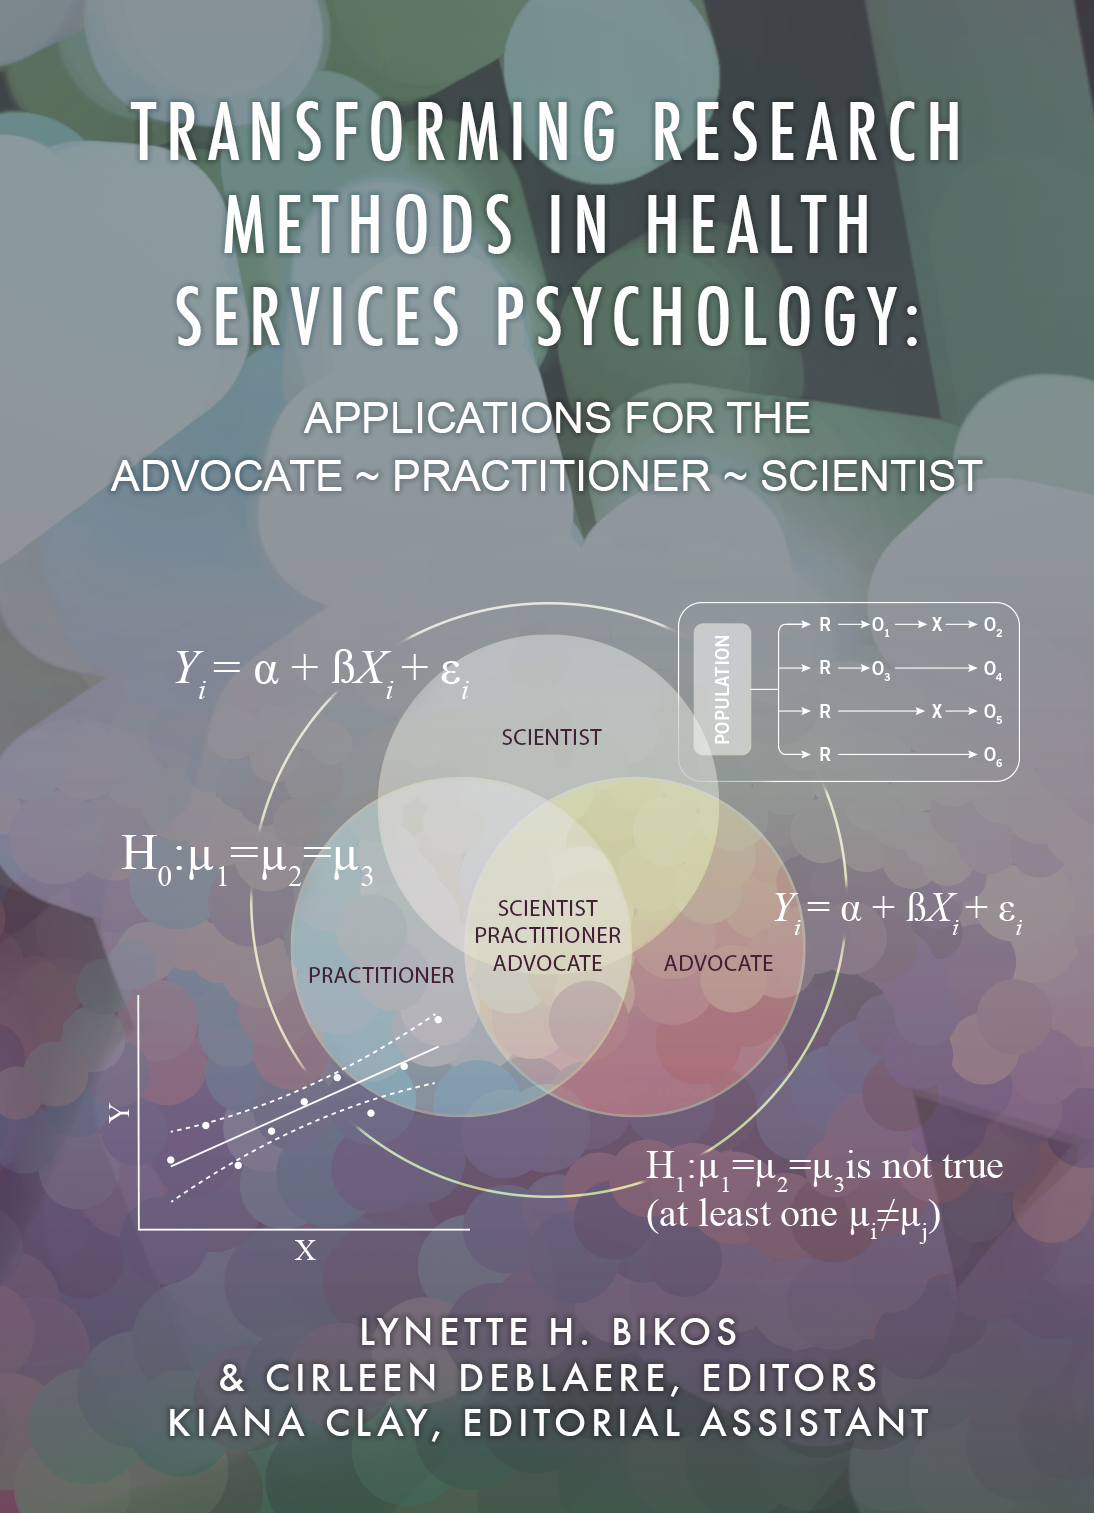
\includegraphics{images/bookcover.png}
\caption{An image of the book cover. Description to follow}
\end{figure}

\hypertarget{writing-empirical-manuscripts}{%
\chapter*{WRITING EMPIRICAL MANUSCRIPTS}\label{writing-empirical-manuscripts}}
\addcontentsline{toc}{chapter}{WRITING EMPIRICAL MANUSCRIPTS}

\hypertarget{APAstyle}{%
\chapter{The APA Style Manuscript}\label{APAstyle}}

\href{https://spu.hosted.panopto.com/Panopto/Pages/Viewer.aspx?pid=8ca9d96d-0ff6-4068-a570-ac290189a4d4}{Screencasted Lecture Link}

This lesson focuses on APA style. While a significant portion of the material focuses on the mechanics of APA style, I also consider:

\begin{itemize}
\tightlist
\item
  APA style as epistemology -- and its relationship with power, privilege, and racism.
\item
  JARS: Journal Article Reporting Standards
\item
  Section by section
\item
  Consideration of writing as a developmental process that occurs throughout grad school and into the profession
\item
  Stylistic issues
\item
  Hallmarks of APA style
\item
  Reducing bias
\end{itemize}

\hypertarget{navigating-this-lesson}{%
\section{Navigating this Lesson}\label{navigating-this-lesson}}

There is about 1 hour and 45 minutes of lecture.

The R markdown file used to create this lecture as well as all of the figures are available at the \href{https://github.com/lhbikos/ReC_Topics}{OER's GitHub site}.

\hypertarget{learning-objectives}{%
\subsection{Learning Objectives}\label{learning-objectives}}

Learning objectives from this lecture include the following:

\begin{itemize}
\tightlist
\item
  Identify the cultural characteristics of APA style.
\item
  Identify two ways that Thompson (2004) has suggested that APA style perpetuates Whiteness and patriarchy in the academy.
\item
  List the components of an abstract.
\item
  Describe why JARS matters.
\item
  Begin memorizing the minutia of APA Style for writing empirical manuscripts/journal articles (no particular order).
\end{itemize}

\hypertarget{readings-resources}{%
\subsection{Readings \& Resources}\label{readings-resources}}

In preparing this chapter, I drew heavily from the following resource(s). Other resources are cited (when possible, linked) in the text with complete citations in the reference list.

\begin{itemize}
\tightlist
\item
  American Psychological Association. (2020). \emph{Publication manual of the American Psychological Association: The official guide to APA style. (Seventh edition.).} American Psychological Association.

  \begin{itemize}
  \tightlist
  \item
    I'm guessing you'll use this more days than not, for the rest of your education.
  \end{itemize}
\item
  Tran, A. G. T. T., \& Lee, R. M. (2014). You speak English well! Asian Americans' reactions to an exceptionalizing stereotype. \emph{Journal of Counseling Psychology, 61}(3), 484--490. \url{https://doi.org/10.1037/cou0000034}

  \begin{itemize}
  \tightlist
  \item
    I use this article in several analyses in the ANOVA series as well as in this lesson when I compare/contrast it to the requirements of APA Style. This article was pubbed in 2014; but I will compare it to the 7th edition (2019) standards.
  \end{itemize}
\item
  Cooper, H. (2020). \emph{Reporting quantitative research in psychology: How to meet APA style journal article reporting standards (Second edition, revised.).} American Psychological Association. \url{https://alliance-primo.hosted.exlibrisgroup.com/permalink/f/rpqmv/CP71332049420001451}

  \begin{itemize}
  \tightlist
  \item
    The e-text version of this may be available at your library. This resource offers section-by-section instruction of the reporting standards and provides numerous examples of writing APA empirical manuscripts.
  \end{itemize}
\item
  Madigan, R., Johnson, S., \& Linton, P. (1995). The language of psychology: APA style as epistemology. American Psychologist, 50(6), 428--436. \url{https://doi.org/10.1037/0003-066X.50.6.428}

  \begin{itemize}
  \tightlist
  \item
    Madigan et al.~(1995) argued that as we learn APA style we are inculcating the professional values of our discipline (and we do this without awareness).
  \end{itemize}
\item
  Thompson, A. (2004). Gentlemanly Orthodoxy: Critical Race Feminism, Whiteness Theory, and the APA Manual. \emph{Educational Theory, 54}(1), 27--57. \url{https://doi.org/10.1111/j.0013-2004.2004.00002.x}
\item
  Critiquing the 5th edition of the style manual (we're now on the 7th) Thompson (2004) pointed out how aspects of APA style contribute to preserving Whiteness.
\item
  Appelbaum, M., Cooper, H., Kline, R. B., Mayo-Wilson, E., Nezu, A. M., \& Rao, S. M. (2018). Journal article reporting standards for quantitative research in psychology: The APA Publications and Communications Board task force report. \emph{American Psychologist, 73}(1), 3--25. \url{https://doi.org/10.1037/amp0000191}

  \begin{itemize}
  \tightlist
  \item
    Yet another copy of the most current JARS. You can also find them in the style manual and on their own website: \url{https://apastyle.apa.org/jars/glossary}
  \end{itemize}
\item
  \emph{White Supremacy Culture.} (n.d.). DRworksBook. Retrieved August 8, 2020, from \url{https://www.dismantlingracism.org/white-supremacy-culture.html}

  \begin{itemize}
  \tightlist
  \item
    Identifies characteristics of White Supremacy Culture in organizations (often used to describe academia).
  \end{itemize}
\end{itemize}

\hypertarget{apa-style-as-epistemology-or-worse}{%
\section{APA Style as Epistemology (or Worse)}\label{apa-style-as-epistemology-or-worse}}

A 1995 article \citep{madigan_language_1995} in the American Psychologist compared APA style to that of other disciplines (history, literary criticism) and argued that APA Style is its own writing genre characterized by (among other things):

\begin{itemize}
\tightlist
\item
  A story schema: introduction, method, results, discussion
  -- Seems so linear; but this is rarely the case (research is messy)
\item
  A depersonalized language of disagreement that focuses on the empirical process and away from investigators as individuals (e.g., ``The primary criticism is that the threshold-setting procedures used in previous experiments are not adequate to ensure that\ldots{}''). The goal is a collaborative, cumulative endeavor based on research data.
\item
  Hedged conclusions: balancing a need to have substantive conclusions that do not extend beyond the data. We use the words, ``tend,'' ``suggest,'' and ``may.'' See Table1.
\item
  A system of headings/subheadings (rather than narrative transitions)
\item
  Paraphrasing rather than directly quoting other works.
  -- Giving authors more flexibility in representing others' perspectives.
\item
  Multiple authors (perhaps contributing to ``more subdued prose'').
\item
  Heavy use of citations introduction and discussion so that the research is placed within an ongoing stream of empirical studies.
\item
  Language that ``does not call attention to itself.'' It can be described as: self-effacing and low-profile.
\end{itemize}

The style manual has grown from its 7-page writers guide in the Psychological Bulletin (1929) to 427 in the 7th edition (2019), today. Madigan et al. \citeyearpar{madigan_language_1995} suggests that the process of mastering APA style, one is enculturated into psychology. That is, we learn APA style -- we inculcate empiricist values (i.e., ``unarticulated practices that reflect fundamental attitudes and values of psychologists'' (p.~428). As such, APA style is epistemological.

Nearly a decade later, Thompson \citeyearpar{thompson_gentlemanly_2004} examined APA style through the lens of critical race feminism and Whiteness Theory. Thompson argued that the expectations regarding clarity precision, appropriateness, sensitivity, and objectivity likely contribute to the academy's investments in Whiteness and patriarchy. While her focus was on APA Style, she suspected that her critique would generalize to other style guides (e.g., Chicago, MLA).

Thompson's \citeyearpar{thompson_gentlemanly_2004} article focused around the gender/sexuality and race values codified by the APA manual (at the time of her article it was the 5th edition). She conducted an analysis of its \emph{power and property investments} and organized her arguments in five themes:

\textbf{Property Rights}: PWIs have treated refereed scholarship (but not indigenous or community knowledge) as intellectual property, demarcated with a certain class. That is, individuals ``own knowledge.'' Evidence includes:

\begin{itemize}
\tightlist
\item
  Using last names as a shorthand reference for work (e.g., ``Dik \& Duffy's 2012 CVQ'').
\item
  Tendency to cite own work rather than say, ``When I previously said\ldots{}''
\item
  The style manual indicates that principal authorship and order of authorship credit should reflect the relative contributions of persons involved (7th ed, APA 1.22) and that relative status should not determine authorship order. Thompson argued that power dynamics (especially around race and gender) likely interfere with this principle.
\item
  The 7th edition has reduced citations of articles with three and more articles to ``First author et al., YEAR'' for all citations.\\
\item
  Regarding, ownership of knowledge -- does it belong to the researcher or the community from which it came? Community knowledge can be studied but not cited. And what about institutions. What if knowledge came from the Black Church? How does one cite that?
\end{itemize}

\textbf{Precedent and pedigree}: In the social sciences, we are expected to cite and give credit to relevant earlier works. Knowledge is seen as cumulative. Citations are essential.

\begin{itemize}
\tightlist
\item
  No ``unhedged statement'' (p.~45) is made without a citation; and in introductory sections, citations are often included with claims that seem obvious! This establishes the requisite lineage.
\item
  Self-citations, expected citations (of the gurus), citations of colleagues exist IN TENSION with a citation economy (page limits, afterall).
\item
  The requirement that scholars locate their project in the context of the existing peer-reviewed literature serves to keep out ideas/projects that would be challenging to the existing power structure.
\end{itemize}

\textbf{Proceduralism}: APA authors learn to address an audience unmarked (as if they were white, male, heterosexual) by gender or race as a ``sign of professionalism'' (p.~48).

\begin{itemize}
\tightlist
\item
  Standardized Format: a four section structure: Introduction, Method, Results Discussion; it could be that the experiences of marginalized and oppressed groups cannot be captured by this scientific narrative structure.
\item
  Standardized Style: prizing scientific appearance and elegance. Thompson (2004) follows the guidelines regarding the use of the ``slash'' (/) and how it is impossible to standardize to the degree that it works for all groups.

  \begin{itemize}
  \tightlist
  \item
    The ``First author et al., (year)'' citation contributes to both gender- and color-blindness. ON the one hand is it ``fair.'' On the other hand, it obscures the person of the author.
  \item
    APA's prohibition against footnotes minimizes ``the good stuff'' (the most juicy arguments are always in the footnotes).
  \end{itemize}
\end{itemize}

\textbf{Protocol}: Propriety or protocol represents conduct that signifies one's understanding of prevailing relations of power, authority and legitimacy.

\begin{itemize}
\tightlist
\item
  The style manual (7th ed, Chapter 5, e.g., 5.2) acknowledges the importance of sensitivity and the avoidance of pejoratives to reference groups of people. Thompson indicates that this is ``admirable'' it fails to address unequal power relations. Further, distinctions between what is insensitive and pejorative may be invisible to those in positions of privilege.
\end{itemize}

\textbf{The gentleman's agreement}: APA style is characterized ``language that conveys professionalism and formality'' (7th ed, 4.7, 4.8) and ``differences should be presented in a professional and noncombative manner'' (7th ed, 4.7).

\begin{itemize}
\tightlist
\item
  Thompson \citeyearpar{thompson_gentlemanly_2004} is concerned that while this is offered with the hope of pluralism and the creation of safe spaces, it causes controversies to be ignored or dismissed and may bolster complicity in racism.
\end{itemize}

\hypertarget{as-we-dive-into-the-specifics}{%
\section{As We Dive into the Specifics}\label{as-we-dive-into-the-specifics}}

Please keep the perspectives of these authors in mind.

Let's also look at the characteristics of White Supremacy Culture in organizations \citep{noauthor_white_nodate}. As we tour through the components of APA style, what resonates with this list? Refer to the .pdf handout or website for more definitions, descriptions, examples, and antidotes.

\begin{itemize}
\tightlist
\item
  Perfectionism

  \begin{itemize}
  \tightlist
  \item
    Perfectionistic culture
  \item
    Worship of the written word
  \item
    Only one right way
  \item
    Either/or thinking
  \end{itemize}
\item
  Concentration of power

  \begin{itemize}
  \tightlist
  \item
    Power hoarding
  \end{itemize}
\item
  Paternalism

  \begin{itemize}
  \tightlist
  \item
    Defensiveness
  \end{itemize}
\item
  Right to comfort

  \begin{itemize}
  \tightlist
  \item
    Fear of open conflict
  \end{itemize}
\item
  Individualism

  \begin{itemize}
  \tightlist
  \item
    I'm the only one
  \end{itemize}
\item
  Progress is more/bigger

  \begin{itemize}
  \tightlist
  \item
    Objectivity
  \item
    Quantity over quality
  \item
    Sense of urgency
  \end{itemize}
\end{itemize}

\hypertarget{the-jars-the-core-of-apa-style}{%
\section{The JARS: The Core of APA Style}\label{the-jars-the-core-of-apa-style}}

The JARS {[}Journal Article Reporting Standards; \citet{appelbaum_journal_2018}{]} were first introduced in a 2008 feature in the American Psychologist \citep{noauthor_reporting_2008} and were included in the 6th edition of the style manual. The updated JARS, published in 2018, expanded the types of quantitative research (JARS-Quant) and included standards for reporting qualitative (JARS-Qual) and mixed methods (JARS-Mixed). Chapter 3 of the 7th edition is devoted to JARS. It contains numerous tables, definitions/explanations, and a flowchart.

The JARS are an attempt to represent what is common across approaches. There is a recognition that specialties/sub-specialties use different terminology. The terms, therefore, should be treated as placeholders and be updated to reflect the various research traditions.

In each of the sections below, I list both the APA style recommendations and JARS elements -- which are somewhat annoyingly separate, adjacent, and overlapping.

In the next section I used text-citations to also refer to the section numbers of the 7th edition of the APA style manual. Additionally, because this OER is publicly available (i.e., not just used in my classroom), I have not copied the JARS elements into this document. They are freely available \href{https://apastyle.apa.org/jars/quantitative}{here}

\hypertarget{title-authorship-author-note-apa-2.3}{%
\subsection{Title, Authorship, Author Note (APA 2.3)}\label{title-authorship-author-note-apa-2.3}}

QUIZLET:
A manuscript title should

\begin{enumerate}
\def\labelenumi{\alph{enumi}.}
\tightlist
\item
  Use abbreviations whenever possible
\item
  Contain at least 30 words
\item
  Be fully explanatory when standing alone
\item
  Begin with the words, A Study of
\end{enumerate}

The title page of a manuscript includes the

\begin{enumerate}
\def\labelenumi{\alph{enumi}.}
\tightlist
\item
  Author's name
\item
  Author's institutional affiliation'
\item
  Running head
\item
  Short title
\item
  All of the above
\end{enumerate}

\hypertarget{title-apa-2.4}{%
\subsubsection{Title (APA 2.4)}\label{title-apa-2.4}}

\begin{itemize}
\tightlist
\item
  Concise statement of main topic of the research,
\item
  Identify the variables or theoretical issues under investigation (and the relationship between t Addhem),
\item
  Focused and succinct (no prescribed word or character limit per the style manual; but a journal might have one).
\item
  Avoid empty words/phrases like ``A study of,'' ``An investigation of''
\end{itemize}

\emph{The lecture further reviews JARS elements.}

\hypertarget{authorshipbyline-apa-2.5-affiliation-apa-2.6}{%
\subsubsection{Authorship/Byline (APA 2.5) \& Affiliation (APA 2.6)}\label{authorshipbyline-apa-2.5-affiliation-apa-2.6}}

\begin{itemize}
\tightlist
\item
  Primary contributors;
\item
  Institutional affiliation AT THE TIME of the study, no more than 2 institutional affiliations (and they both need to have contributed equally)
\item
  Very specific style guidelines (with superscript notations) for connecting authors and their affiliations
\item
  In the order of contribution -- lots of ethical, practical, and sensitive considerations about who gets to be an author and in what order.
\end{itemize}

\textbf{Sticky Issues about Authorship}

\begin{itemize}
\tightlist
\item
  Faculty as first authors
\item
  Ongoing projects with years of investment sponsored by faculty
\item
  Who gets ``the call''?
\item
  Order between equal contributors (e.g., Singer \& Willett)
\item
  In equal contributions it's ok (not ideal) to mention in the author note
\item
  GOAL: name on a project, less concerned about author order
\item
  Generally, graduate projects include the faculty sponsor as an author (last at SPFC conference; likely elsewhere at professional conferences or publication)
\item
  Author-order rubrics can be useful to guide the decision
\end{itemize}

\hypertarget{author-note-apa-2.7}{%
\subsubsection{Author Note (APA 2.7)}\label{author-note-apa-2.7}}

Place the author note at the bottom half of title page. There are more specific instructions in style manual. Generally author note has four paragraphs:

\begin{itemize}
\tightlist
\item
  ORCID iDs \url{https://orcid.org}
\item
  Changes in affiliation subsequent to the time of the study, ``{[}Author's name{]} is now at {[}new affiliation{]}.'' Can also be used if an author is deceased.
\item
  Disclosures and acknowledgements (i.e., study registration, open practices and data sharing, related reports, conflicts of interest, financial or other assistance).
\item
  Contact information for corresponding author. Requires full name, complete mailing address, and e-mail. Prescribed format: Correspondence concerning this article should be addressed to {[}author's name'{]}, {[}complete mailing address{]}. Email: \href{mailto:author@institution.edu}{\nolinkurl{author@institution.edu}}
\end{itemize}

\emph{The lecture further reviews JARS elements.}

\hypertarget{running-head-apa-2.8}{%
\subsubsection{Running Head (APA 2.8)}\label{running-head-apa-2.8}}

\begin{itemize}
\tightlist
\item
  Abbreviated title printed at the top of the pages of a ms or pubbed article to identify it for the readers
\item
  Max of 50 characters (counting letters, punctuation, spaces between words). If the title is already 50 characters or fewer, the full title can be sued. Avoid abbreviations in the running head, although the ampersand can be swapped (\& for ``and'').
\item
  Appears flush left in all uppercase letters at the top of the title and subsequent pages
\end{itemize}

\hypertarget{manuscript-page-headerspage-numbers-apa-8.03}{%
\subsubsection{Manuscript Page Headers/Page Numbers (APA 8.03)}\label{manuscript-page-headerspage-numbers-apa-8.03}}

\begin{itemize}
\tightlist
\item
  Number consecutively, beginning with the title
\item
  Identify each page with the running head along with the page number
\item
  To facilitate a blinded review, do not include your name in these
\item
  Use the automatic functions of the word-processer to generate page headers and page numbers
\end{itemize}

\hypertarget{abstract-apa-2.8-3.3}{%
\subsection{Abstract (APA 2.8, 3.3)}\label{abstract-apa-2.8-3.3}}

QUIZLET:
An abstract should

\begin{enumerate}
\def\labelenumi{\alph{enumi}.}
\tightlist
\item
  Appear on the same page above the title and introduction
\item
  Be single-spaced and set with larger margins
\item
  Begin on page 2
\item
  Be no longer than 3\% of the text
\end{enumerate}

Abstract lengths vary from journal to journal; the typical range is from \_\_\_ to\_\_\_ words.

For real\ldots a good abstract is:

\begin{itemize}
\tightlist
\item
  Concise and specific
\item
  Nonevaluative
\item
  Coherent and readable
\item
  Loaded with keywords
\item
  May be a single paragraph (no indentation of first line) or structured (still no indentation, but labels inserted for the prescribed sections).
\end{itemize}

\hypertarget{recipe-for-an-abstract}{%
\subsubsection{Recipe for an Abstract}\label{recipe-for-an-abstract}}

\begin{itemize}
\tightlist
\item
  Identify the problem under investigation (1 sentence)
\item
  Identify the participants and salient characteristics
\item
  Identify the experimental method, including the apparatus, data gathering procedures, complete test names, etc.
\item
  Identify findings (including statistical significance levels)
\item
  Identify conclusions and implications/applications.
\item
  Avoid \emph{boilerplate} sentences.
  -- At the end of an abstract, I often read, ``Findings and implications will be discussed.'' This is boilerplate because ``everyone says it.'' It's also empty and a waste of words because it tells us NOTHING about the study.
\item
  The style manual includes outlines for a variety of types of manuscripts.
\end{itemize}

\emph{The lecture further reviews JARS elements.}

\hypertarget{keywords}{%
\subsubsection{Keywords}\label{keywords}}

Keywords include single words, phrases, or acronyms that describe the most important aspects of the paper. The purpose is indexing in databases (it's what we search on in database like PsychInfo).

\hypertarget{introduction-apa-2.11}{%
\subsection{Introduction (APA 2.11)}\label{introduction-apa-2.11}}

QUIZLET:
The introduction section of a research report should:

\begin{enumerate}
\def\labelenumi{\alph{enumi}.}
\tightlist
\item
  Include a thorough historical review of the literature
\item
  Define all of the terms that would be unintelligible to a reader with no previous exposure to the field
\item
  Present the specific problem to be explored and described in the research strategy
\item
  Be clearly labeled.
\end{enumerate}

What question should the introduction section of a research report attempt to answer?
a. What are the theoretical implications of the current research?
b. What is the point of the study?
c.~What is the logical link between the problem and the research strategy?
d.~All of the above are correct.
e. Only a and c of the above are correct.

Before you write, consider this:

\begin{itemize}
\tightlist
\item
  Why is this problem important?
\item
  How does this study link to previous work?
\item
  What are the primary/secondary hypotheses/objectives? What are their links to theory?
\item
  How do the hypotheses and research design relate to each other?
\item
  What are the theoretical and practical implications?
\end{itemize}

Three parts to the Introduction

\begin{itemize}
\tightlist
\item
  Brief introduction, 1-2 paragraphs
\item
  Review of relevant scholarship, 1-2 pages
\item
  Purpose, rational, hypotheses, 1-2 paragraph's at the section's close.
\end{itemize}

\hypertarget{the-brief-introduction}{%
\subsubsection{The Brief Introduction}\label{the-brief-introduction}}

A good introduction paragraph answers the following questions in 1-2 paragraphs

\begin{itemize}
\tightlist
\item
  What is the point of the study?
\item
  How do the hypothesis and experimental design relate to the problem?
\item
  What are the theoretical implications of the study and how does the study relate to previous work in the area?
\item
  What are the theoretical propositions tested and how were they derived?
\end{itemize}

In the middle\ldots above ALL

\begin{itemize}
\tightlist
\item
  Demonstrate that the problem is IMPORTANT
\item
  Narrative thread.
\item
  Always refer to the THEORETICAL BACKGROUND
\item
  Narrative thread.
\item
  Closing paragraph a statement of purpose and rationale of project.
\item
  Narrative thread.
\end{itemize}

The closing paragraph(s) of the Introduction

\begin{itemize}
\tightlist
\item
  What variables did I plan to manipulate?
\item
  What results did I expect and why did I expect them? (the logic of this should also be made clear)
\item
  What is my rationale for each hypothesis?
\end{itemize}

\emph{The lecture further reviews JARS elements.}

\hypertarget{bikos-developmental-perspective-on-learning-to-write-the-empirical-manuscript}{%
\subsubsection{Bikos' Developmental Perspective on Learning to Write the Empirical Manuscript}\label{bikos-developmental-perspective-on-learning-to-write-the-empirical-manuscript}}

Over the years I have been learning writing skills of my own and, in my roles as instructor and peer reviewer, providing feedback to others. Below is an oversimplified model of what I think I'm observing as students and scholars learn to write empirical manuscripts (in the specific APA style).

Figure 1. The first stage of writing.

\begin{figure}
\centering
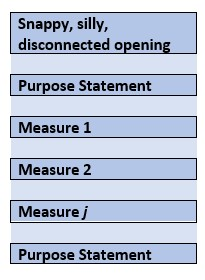
\includegraphics{images/APAstyle/Stage1.jpg}
\caption{Image of the first stage of writing}
\end{figure}

Figure 2. The second stage of writing.

\begin{figure}
\centering
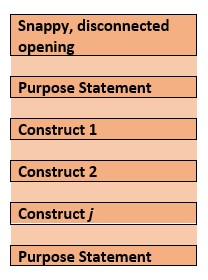
\includegraphics{images/APAstyle/Stage2.jpg}
\caption{Image of the second stage of writing}
\end{figure}

Figure 3. The third stage of writing.

\begin{figure}
\centering
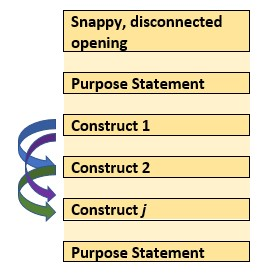
\includegraphics{images/APAstyle/Stage3.jpg}
\caption{Image of the third stage of writing}
\end{figure}

Figure 4. The fourth stage of writing.

\begin{figure}
\centering
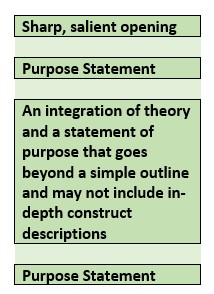
\includegraphics{images/APAstyle/Stage4.jpg}
\caption{Image of the fourth stage of writing}
\end{figure}

\hypertarget{perennial-notes-from-research-project-faculty-graders}{%
\subsubsection{Perennial Notes from Research-Project Faculty Graders}\label{perennial-notes-from-research-project-faculty-graders}}

\begin{itemize}
\tightlist
\item
  Start with your problem statement
  -- What is your DV and why does the reader care?
\item
  Theory must drive your model/manuscript.
  -- ``A list of variables does not a theory-driven model make.''
\item
  Active headers are your friends
  -- Not helpful: ``Gender \& RSB''
  -- More helpful: ``RSB vary across Genders''
\end{itemize}

\hypertarget{method-apa-2.06-chapter-3}{%
\subsection{Method (APA 2.06; Chapter 3)}\label{method-apa-2.06-chapter-3}}

\begin{itemize}
\tightlist
\item
  Describes in detail how the study was conducted.
\item
  Includes conceptual and operational definitions of variables.
\item
  How much info is enough? Readers must be able to\ldots{}
  -- Evaluate the appropriateness of the method
  -- Judge the reliability and validity of your results
  -- Replicate the study
\end{itemize}

Many of the JARS elements have even more detail in the text that follows the table. In your first few papers, make sure to review and imitate.

\emph{The lecture further reviews JARS elements.}

Regarding these tables -- flowchart and tables in style manual, Appelbaum (2018) article, or \href{https://apastyle.apa.org/jars/jars-quant-decision-flowchart.pdf}{website}.

\hypertarget{results-discussion-chapter-3}{%
\subsection{Results \& Discussion (Chapter 3)}\label{results-discussion-chapter-3}}

\emph{The lecture references the JARS elements in detail.}

Section 6.43 of the APA style manual details the basic form for statistical output (``statistical strings''); 6.44 provides statistical abbreviations and symbols.

\hypertarget{headings-apa-2.7}{%
\subsection{Headings (APA 2.7)}\label{headings-apa-2.7}}

The 7th edition of the style manual updated the levels of headings. The change is to the L3 heading -- making it a little easier for Word processing programs.

There are now 5 levels of headings. A useful table that illustrates them can be found \href{https://apastyle.apa.org/style-grammar-guidelines/paper-format/headings}{here}.

Headings follow a top-down progression.

\begin{itemize}
\tightlist
\item
  Each section (i.e., Title {[}on first page{]}, Method, Results, Discussion) starts with an L2 heading.
\item
  Do not include an ``Introduction'' heading -- the first paragraphs of a paper are automatically expected to be introductory in nature.
  Here's the heading structure in the paper (a ``brief report'') we are investigating:
\end{itemize}

\textbf{You Speak English Well! Asian American's Reactions to an Exceptionalizing Stereotype Microaggressions Against Asian Americans} (L1, centered, bold, title case)

\textbf{Method} (L1, centered, bold, title case)

\textbf{Sample} (L2, flush left, bold, title case)
\textbf{Procedure and Materials} (L2, flush left, bold, title case)
\textbf{Analysis and Manipulation Check} (L2, flush left, bold, title case)

\textbf{Results} (L1, centered, bold, title case)

\textbf{Discussion} (L1, centered, bold, title case)

\textbf{Conclusion} (L1, centered, bold, title case)

\hypertarget{reference-list}{%
\subsection{Reference List}\label{reference-list}}

The reference list should start on a new page with ``References'' in bold and centered (an L1 heading -- like the title).

The general format of the reference is: Author (Date). Title. Source. The 7th edition has made significant improvements in making this format consistent throughout the many types of references. Plus, Chapter 9 in the 7th edition has a number of tools for problematic reference entries.

One substantial change in the 7th edition is the immediate use of ``et al.'' after the first author's name there are three or more authors. In contrast, up to 20 authors can be included in the entry in the reference list.

Use a hanging indent and format this with the paragraph-formatting function of your word processor's ruler. This means that the first line of each reference is flush left and subsequent lines are indented by 0.5 inches:

The text-citations and reference lists must be 100\% consistent. If you have consistently (and properly) used your reference management system, this will happen by magic. Even so, one of the last things I do is a text-ref/ref-list cross check. I open 2 copies of the manuscript and put them side-by-side on the monitor. Starting with the text (and in track changes), each time I come to a reference, I put an X in front of it on the ref list. I go through the entire document. If there are items in the ref list missing, I note it (then add it). If there are additional references in the ref list that I haven't checked, I do a quick search to see if they are really missing, and if so, I delete them. For dissertation proposals and defenses, we ask first and second year students to do this for us -- it familiarizes them with RVT topics, the dissertation process, and the literature.

Because of Zotero, Mendeley, RefWorks, EndNote, and other reference management systems (as well as the good tools in the style manual), I won't say more about text-citations and reference lists.

\hypertarget{stylistic-issues-apa-chapter-4-on-writing-style-and-grammar}{%
\subsection{\texorpdfstring{Stylistic Issues (APA Chapter 4 on \emph{Writing Style and Grammar})}{Stylistic Issues (APA Chapter 4 on Writing Style and Grammar)}}\label{stylistic-issues-apa-chapter-4-on-writing-style-and-grammar}}

APA (4.0) is committed to a literary style characterized by continuity (logical consistency of expression throughout a written work), flow (smooth cadence of words and sentences), conciseness (say only what you need to say), and clarity. I encourage the authors to read Chapter 4 of the style manual for examples of how to increase the effectiveness with which they write.

\begin{itemize}
\tightlist
\item
  Transitional words between sentences and phrases (or sentences) between paragraphs and sections assist with continuity and flow
  -- Time: then, next, after, while, since
  -- Cause-effect: therefore, consequently, as a result
  -- Addition links: in addition, moreover, furthermore, similarly
  -- Contrast links: but, conversely, nevertheless, however, although
  -- Think twice about using adverbs (certainly, consequently, importantly, interestingly) as transition words.
\item
  Active headings/subheadings contribute to continuity and flow.
\item
  Don't add any more words than necessary. Say \emph{only} what needs to be said:
  -- No ``fluff'' (avoid: very, really)
  -- Maintain a professional tone (avoid cliché's, rhymes, alliteration, metaphors, slang -- remember a global audience)
\item
  Clarity is improved with a varied sentence length; long sentences can be confusing.
\item
  APA style permits both active (subject, verb, object: ``students completed surveys) and passive (object of verb is presented first: ``surveys were completed by students'') voice. The active voice contributes to direct, clear, and concise statements.
\end{itemize}

More style-congruent advice:
* Avoid abstract stacking.
* Avoid organizing by an author(s)' name(s).
-- Organize by ideas -- Unless it is important, citations should be at the end of a sentence. Ask yourself why you are starting a sentence with an author's name -- Is he or she the point of your sentence? Could be but most likely not.
* Use quotations sparingly: short ones, infrequently.
* Precision, continuity, clarity, efficiency (stop with the long sentences)
* Active voice (``It'' is banned as first word in paragraphs and sentences).
* Manuscript must be written in first person.
-- Avoid this: ``Hypotheses for the present study included\ldots{}''
-- Do this instead: ``In our study, we hypothesized\ldots{}''
* Past tense or present perfect tense for the literature review, method, and results sections; present tense for the discussion section.

\hypertarget{reducing-bias-apa-chapter-5}{%
\subsection{Reducing Bias (APA Chapter 5)}\label{reducing-bias-apa-chapter-5}}

Chapter 5, ``Bias-Free Language Guidelines'' is new to the 7th edition. A big message is that this is-and-will-continue-to-be-evolving.

Here are some of the highlights

\begin{itemize}
\tightlist
\item
  Describe relevant characteristics; it is likely unnecessary to collect and/or report on all personal characteristics for the topic being explored.
\item
  Don't shy away/hide/gloss over actual differences in the target population from the general population. Describe them clearly and professionally.
\item
  There are specific guidelines for level of specificity in labels/language for various topics (e.g., disability, age, gender identity, race/ethnicity/nationality, sexual orientation, SES). Look them up.
\item
  A few guiding principles (but there are so many more\ldots read the chapter):
  -- Call people what they call themselves (especially in qualitative or participant-informed research designs). Also recognize that no group is monolithic so there may be within-group differences about this.
  -- Accept that language changes with time -- stay open minded.
  -- There is debate about person-first language (``a child with autism'') and identity-first language (``an autistic child''). Get consultation and listen to the research participants.
  -- ``White,'' ``cis-gendered,'' ``heterosexual,'' and ``U.S.'' is often the standard against which others are judged. This centers Whiteness. Avoid these false hierarchies. When these comparisons are made, placing the socially dominant group on the left side of a graph or at the top of a table may imply these groups are the universal standard.
\end{itemize}

A (very) few specific details:
* On identification of race:
-- ``African American'' is discouraged as an umbrella term for people of African ancestry worldwide because it obscures other ethnicities or national origins (e.g, Jamaica). In these cases use Black (with a capital ``B'').
-- ``Caucasian'' is discouraged as an umbrella term for White or European because it originated as a way of classifying White people as a superior race. Use White (with a capital ``W'').
-- ``Native American'' and ``Native North American'' seem to be preferred in North America.
-- ``Latin@'' is now widely accepted for Latino and Latina; as is ``Latino/a.'' ``Latinx'' can also be used as a gender-neutral or nonbinary term inclusive of all genders.\\
* Avoid writing about ``minorities.'' Terms like ``people of color'' or ``underrepresented groups'' are preferred. Do not assume that members of any of these groups are ``underprivileged.'' Terms like ``economically marginalized'' or ``economically exploited'' may be preferred.
* Use ``sexual orientation'' not ``sexual preference,'' ``sexual identity,'' or ``sexual orientation identity.'' The term ``sexual and gender minorities'' refers to multiple sexual and/or gender minority groups or write about ``sexual orientation and gender diversity.''\\
-- LGBT is considered outdated, but LGBTQ, LGBTQ+, LGBTQIA, AND LGBTQIA+ may be used to refer to multiple groups (but be careful and specific; if you are researching transgender people\ldots then talk about transgender people).
* ``They'' is now acceptable to use in the singular. There are a number of circumstances when this is recommended. A few include:
-- When it is the person's preferred pronoun.
-- When the pronoun is unknown.
-- In place of ``he or she,'' ``s/he,'' and ``(s)he.''

\hypertarget{closing-thoughts}{%
\subsection{Closing Thoughts}\label{closing-thoughts}}

\begin{enumerate}
\def\labelenumi{\arabic{enumi}.}
\tightlist
\item
  Fluency in APA style is a long journey. One of my own strategies in an APA Cheat Sheet (presently 38 pages long).
\end{enumerate}

\begin{enumerate}
\def\labelenumi{\alph{enumi}.}
\tightlist
\item
  I wrote it to help with reviewing/editing/grading (and also for my own writing), so I can search on words/phrases that I'm likely to say.
\item
  I can add/update it.
\item
  Each element in my cheatsheet has the section number (for papers I review as well as my own self-doubt when I wonder, later).
\end{enumerate}

\begin{enumerate}
\def\labelenumi{\arabic{enumi}.}
\setcounter{enumi}{1}
\tightlist
\item
  Having now toured the 7th ed, what are your thoughts about its relation to power, privilege, racism/anti-racism, and White supremacy culture?
\end{enumerate}

Repeated are the characteristics of White supremacy culture. I have italized those that strike me as being reflected in APA Style.

\begin{itemize}
\tightlist
\item
  Perfectionism

  \begin{itemize}
  \tightlist
  \item
    \emph{Perfectionistic culture}
  \item
    \emph{Worship of the written word}
  \item
    \emph{Only one right way}
  \item
    Either/or thinking
  \end{itemize}
\item
  Concentration of power

  \begin{itemize}
  \tightlist
  \item
    \emph{Power hoarding}
  \end{itemize}
\item
  Paternalism

  \begin{itemize}
  \tightlist
  \item
    Defensiveness
  \end{itemize}
\item
  Right to comfort

  \begin{itemize}
  \tightlist
  \item
    \emph{Fear of open conflict}
  \end{itemize}
\item
  Individualism

  \begin{itemize}
  \tightlist
  \item
    I'm the only one
  \end{itemize}
\item
  Progress is more/bigger

  \begin{itemize}
  \tightlist
  \item
    \emph{Objectivity}
  \item
    Quantity over quality
  \item
    Sense of urgency
  \end{itemize}
\end{itemize}

  \bibliography{STATSnMETH.bib}

\end{document}
